\subsection{Typical Behavior}

The previous section asserted that, whatever the model parameters, optimal paths conform to a bracket shape. One might suppose that increasing the width of the obstacle $\sigma$ or the relative cost $A/P$ causes $\yhat$ to increase commensurately, giving the obstacle a wider and wider berth. This dependence is observed for large $\yhat$, but when parameters are tuned to draw the optimal path closer to the origin, it undergoes a discontinuous jump from a finite bracket to the direct path ($\yhat=0$). As an example, consider the path in Figure \ref{fig:gaussian}. When $A/P=?/55$, a long walk around is cheap compared to treading on the origin, and the closest approach $\yhat$=16. (In this simulation, the other parameters were fixed arbitrarily at $n=?$ and $\sigma$=?.) However, when the baseline cost is dialed back such that $A/P=?/56$, the path jumps discontinuously through the origin ($\yhat=0$). Intermediate paths are not cost-effective: at a certain point, what we save by avoiding the dead center is not worth the extra steps.

\begin{figure}
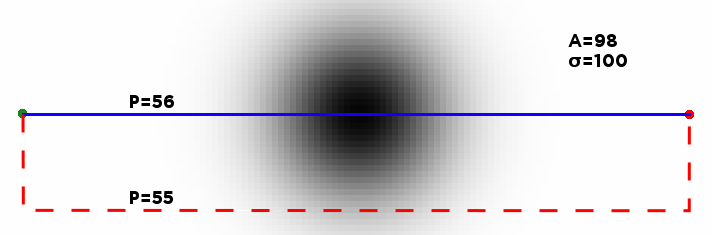
\includegraphics[width=\columnwidth]{graphix/Gaussian.png}
\caption{Gaussian Cost Function - Straight path is optimal when $P=56$, the bracket path when $P=55$. }
\label{fig:gaussian}
\end{figure}

\subsection{Mathematical Explanation}
Our goal is to show why there are certain parameters that result in one of the three behaviors discussed. 
\begin{enumerate}
\item Minimum path cost is at $\yhat=0$
\item Minimum path cost is at finite $\yhat>0$
\item Minimum path cost is infinitely far away. 
\end{enumerate}

The cost of a bracket path in terms of the model parameters and some choice of $\yhat$ is 
\begin{align*}
C(p_{\yhat}) =& C(\text{segment 1}) + C(\text{segment 2}) + C(\text{segment 3}) \\
=&\Big[\yhat P + \sum\limits_{i=0}^{\yhat-1} f(-n, i) \Big] +
         \Big[2nP + \sum\limits_{x=-n}^{n}    f(x,\yhat) \Big]\\
     &+\Big[\yhat P + \sum\limits_{i=0}^{\yhat-1} f(n, i) \Big].
\end{align*}

Now let us assume that we begin far from the obstacle, so $n \gg \sigma$; in this limit, the cost due to the obstacle on segments 1 and 3 is very small compared to the baseline cost and the cost along segment 2.
\begin{equation}
C(p_{\yhat}) \approx (2n+2\yhat)P +  \sum\limits_{x=-n}^{n} f(x,\yhat)
\end{equation}

We are only concerned with the cost of each path in relation to other paths, so we will express the cost of some $p_{\yhat}$ relative to the cost of the direct path like so. 
\begin{align*}
\Delta C(\yhat) =& C(\yhat)-C(0) \\
=& \Big[(2n+2\yhat)P +  \sum\limits_{x=-n}^{n} f(x,\yhat) \Big] \\
 & - \Big[(2n+2(0))P +  \sum\limits_{x=-n}^{n} f(x,0) \Big] \\
=& 2P\yhat + \sum\limits_{x=-n}^{n} \Big[ f(x,\yhat)-f(x,0) \Big]
\end{align*}

When $\Delta C < 0$ for some $\yhat$, the direct path is not optimal.

With a Gaussian obstacle as $f$,
\begin{equation}
\Delta C(\yhat) = 2P\yhat + \sum\limits_{x=-n}^{n} \left[A\exp\left(-\frac{x^2 + \yhat^2}{2\sigma^2}\right) - A\exp\left(-\frac{x^2}{2\sigma^2}\right) \right]
\end{equation}

We have already assumed $n \gg \sigma$, so we can approximate the sum over $x \in [-n, n]$ as the sum over all $x$, which has a simple solution. The tails of the Gaussian contribute negligibly.

\begin{equation}
\sum\limits_{x=-n}^{n} \rightarrow \text{Future Dan will sort this out.}
\end{equation}

Finally, we have a closed-form expression for the cost of bracket path $p_{\yhat}$ compared to the direct path.
\begin{equation}
\Delta C(\yhat) = 2P\yhat + A\sigma\sqrt{2\pi}\left[\exp\left(-\frac{\yhat^2}{2\sigma^2}\right) - 1\right]
\end{equation}

Now, we locate the $\yhat$ that minimize $\Delta C$.
\begin{align}
\frac{d\Delta C}{d\yhat} = 
&2P - \frac{\yhat}{\sigma}A\sqrt{2\pi} \exp\left(-\frac{\yhat^2}{2\sigma^2} \right) = 0 \\
  \frac{P}{A} =& \sqrt{\frac{\pi}{2}} \frac{\yhat}{\sigma} \exp\left(-\frac{\yhat^2}{2\sigma^2} \right)
  \label{eq:PA}
\end{align}
\begin{figure}
\centering
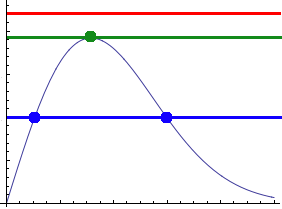
\includegraphics[width=0.4\columnwidth]{graphix/lambert.png}
\caption{Plot of $x \exp(-x^2)$, with lines marking values where the equation has no solutions (top line), one solution (middle line) or two solutions (bottom line).}
\label{fig:lambert}
\end{figure}

The solution for $\yhat$ is related to the Lambert W-function, which is cannot be written in closed form.  Depending on the cost ratio $P/A$, it can admit 0, 1 or 2 solutions, illustrated in Figure \ref{fig:lambert}. We can make several observations.
\begin{enumerate}
\item Eq. \ref{eq:PA} peaks when $\yhat/\sigma = 1$, attaining $P/A=\sqrt{\pi/2e}$. If we set $P$ and $A$ such that $P/A > \sqrt{\pi/2e} \approx 1.57$, there is no solution to Eq. \ref{eq:PA}, and the only minimum of $\Delta C$ occurs on the boundary at $\yhat=0$. The direct path is optimal.
\item When $P=0$, $\Delta C$ has a minimum at infinity. We require a finite baseline cost to keep the solution from running to $y \rightarrow \infty$ before traversing $x$.
\end{enumerate}
\begin{enumerate}
\item Two critical points are necessary for there to be a finite $\yhat>0$, as seen in Figure \ref{fig:twosolutions}. 
\item It is not sufficient to have two critical points to cause a finite $\yhat>0$, since the minimum may not have a negative value, meaning that the optimal path will be at $\yhat=0$. Similar scenario occurs when there is only one critical point as in Figure \ref{fig:inflection}. 
\item If there are no critical points as in Figures \ref{fig:zero} and \ref{fig:infinity}, then the extrema must be at the limits. If $P>0$, you end up with a positive slope like in Figure \ref{fig:zero} and the optimal minimum cost path is at $\yhat=0$. If $P=0$, then you get a negative slope and the minimum value is at $\yhat=\infty$. This follows the intuition where if $P$ is very high, then the straight path is optimal, and if $P=0$, the path length does not matter and the path can be arbitrarily far away. 
\end{enumerate}

\begin{figure}[t]
\centering
\subfloat[Two Critical Points: $\yhat>0$]{
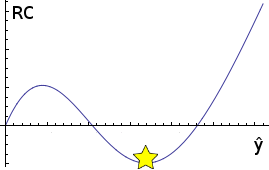
\includegraphics[width=0.4\columnwidth]{graphix/twosolutions.png}
\label{fig:twosolutions}}
\qquad
\subfloat[One Critical Point: $\yhat=0$]{
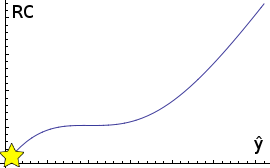
\includegraphics[width=0.4\columnwidth]{graphix/inflection.png}
\label{fig:inflection}}\\
\subfloat[No Critical Points: $\yhat=0$]{
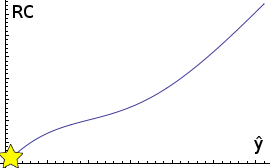
\includegraphics[width=0.4\columnwidth]{graphix/zero.png}
\label{fig:zero}}
\qquad
\subfloat[No Critical Points, $P=0$: $\yhat=\infty$]{
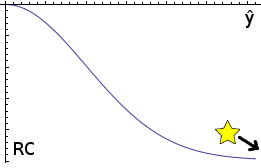
\includegraphics[width=0.4\columnwidth]{graphix/infinity.png}
\label{fig:infinity}}
\caption{Gaussian Relative Costs (y-axis) over different passing distances. Minimum cost/optimal path marked with a star. In (a), the optimum passing distance is at a finite $\yhat>0$. In (b) and (c) the optimum is at $\yhat=0$. In (d), the optimum is as far away as possible. }
\label{fig:globfig}
\end{figure}

